%qqqqqqqqqqqqqqqqqqqqqqqqqqqqqqqqqqqqqqqqqqqqqqqqqqqqqqqqqqqqqqqqqqqqqqqqq
%Quote
\begin{savequote}[50mm]
%‘‘El cosmos es todo lo que es, todo lo que fue y todo lo que será. Nuestras 
%más ligeras contemplaciones del cosmos nos hacen estremecer: Sentimos como 
%un cosquilleo nos llena los nervios, una voz muda, una ligera sensación como
%de un recuerdo lejano o como si cayéramos desde gran altura. Sabemos que nos
%aproximamos al más grande de los misterios.’’
%\qauthor{Carl Sagan}
\end{savequote}
%qqqqqqqqqqqqqqqqqqqqqqqqqqqqqqqqqqqqqqqqqqqqqqqqqqqqqqqqqqqqqqqqqqqqqqqqq




%#########################################################################
\chapter{Teoría sobre AGN}
\label{cha:Theoretical Framework}


Al observa la luz de las galaxias en el óptico e infrarrojo cercano, se ve que es dominado mayormente por estrellas, con una pequeña contribución de polvo y gas. Partiendo del hecho de que el espectro de las estrellas puede ser considerado como un espectro de Plank, el cual depende de la temperatura, la masa y edad estelar. Entonces es posible considerar el espectro de una galaxia como la superposición de espectros  estelares. Bajo esta aproximación se puede además decir, que el espectro de las galaxias sería la superposición de espectros de Plank, definidos en un rango de temperaturas. 

Sin embargo, algunas galaxias presentan anomalías en sus espectros,  mostrando una distribución de energía mucho mayor. Algunas enseñan líneas de emisión en zonas poco comunes, y otras en rangos muy amplios, desde las longitudes de onda del radio hasta rayos-X, y algunas hasta rayos gamma. Ver figura (\ref{fig:Espectro_QSOs}). Estas emisiones se originan en regiones muy centrales de la galaxia, por lo cual se les dio el nombre de Núcleo Activo de Galaxias (AGN's por sus siglas en ingles).

Se considera que el causante de la activación de los AGNs son las interacciones gravitacionales. La interacción debida a la fuerzas de marea o la fusión de galaxias genera una turbulencia en el potencial gravitacional que provoca que el gas empiece a colapsar hacia el centro de la galaxia. 

En la actualidad existe una distinción para los diferentes tipos de  AGN's, un tipo específico son los cuásares. Son objetos muy luminosos, su brillo puede superar por un factor de cien el brillo de su galaxia anfitriona. Los procesos que ocurren al interior de un AGN son los más energéticos en el ámbito de la astrofísica. 


%*************************************************************************
%Introducción a AGN's
\section{Introducción a AGN's}
\label{sec:Introduction_AGN's}
%***********************************************************************

Los AGNs son considerados los motores centrales de las galaxias. Su  actividad nuclear esta patrocinada por la acreción de materia. 

Si se desea profundizar más en la teoría de los AGN's, se recomienda abordar los textos: \cite{schneider2006} y \cite{carroll2007}. Estos fueron los textos en que se baso este capítulo. 


%---------------------------------------------------------------------
	%historia
	\subsection{Historia}
	\label{subsec:History}
%---------------------------------------------------------------------
	
En la época de 1908, se observó que la galaxia NGC 1086 que presentaba fuertes lineas de emisión, que eran poco comunes. En 1943, Carl Seyfert a través de un análisis sistemático pudo identificar una nueva clase de galaxia, las cuales llevan su nombre. Estos núcleos de galaxias activas (Seyferts) presentan un muy alto brillo superficial, y su espectro en la región central esta dominado por fuertes líneas de emisión y de alta extinción.  

Los catálogos 3C y 3CR (Catálogos en infrarrojo). \footnote{Catálogo de observaciones hechas con el Cambridge four-element interferometer a una frecuencia de 159MHz} permitieron encontraron objetos muy puntuales con una muy alta línea de emisión. Esta alta emisión no permitía determinar la forma del objeto central que hospedaba la galaxia. Solo fue cuando se pudieron construir telescopios con un poder de resolución mayor que se pudo ratificar que eran fuentes puntuales. A medida que fue pasando el tiempo y se mejoraron  las observaciones, se empezaron a encontrar más fuentes con estas características. A estos cuerpos se les denomino  Cuásares\footnote{Cuásar viene del ingles Quasars (quasi-stellar radio source)}.

Los cuásares son un tipo específico de AGNs. Sin embargo, una buena forma de conocer las propiedades y arquetipos de  AGN's, es identificando las propiedades de los cuásares. Es por esto que a continuación se presenta una clasificación sobre los diferentes cuásares.  La figura (\ref{fig:Espectro_QSOs}) presenta un espectro típico de AGN, cabe resaltar que dicha imagen es la superposición de espectros de QSOs

\begin{center}
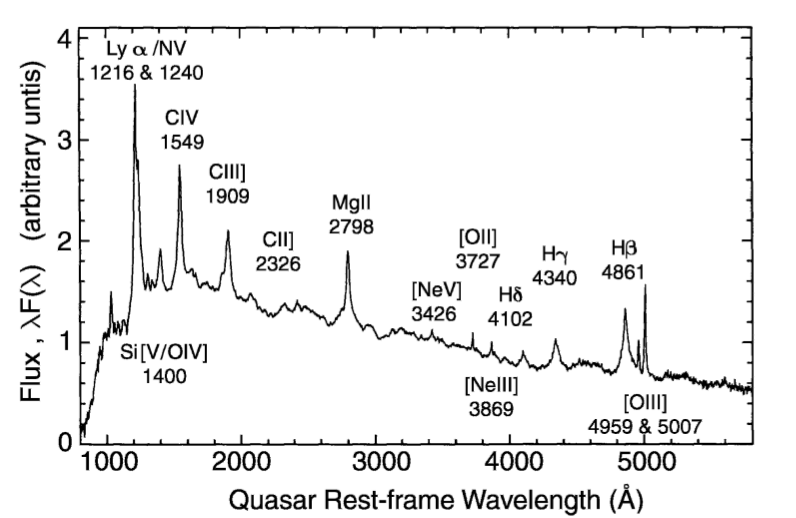
\includegraphics[scale=.3]{./figures/3_AGNs/Espectro_tipico_AGN.png}
\figcaption{\emph{Espectro combinado de varios QSOs, usando las observaciones del Large Bright Quasar Survey \cite{francis1991}.}}\label{fig:Espectro_QSOs}
\end{center}
%---------------------------------------------------------------------
	%M
	\subsection{Propiedades fundamentales de los Cuásares}
	\label{subsec:Fundamental_properties_quasars}
%---------------------------------------------------------------------

Por lo general los cuásares presentan una serie de propiedades que son comunes en varios tipos de AGN's, entre las propiedades se destacan:


- Fueron descubiertos por ser fuentes de radio muy puntual 

- Emite en todas las longitudes de onda, desde el radio a los rayos-X principalmente.

- El flujo de la fuente varía en casi todas las frecuencias y longitudes de onda.

- En general se encuentra que la escala de tiempo de variabilidad es más pequeña y su amplitud más grande, cuando se va ha frecuencias más altas.

- El espectro óptico es muy azul ($U-B < -0.3$). La mayoría de los cuásares presentan un corrimiento a rojo alto  $z \lesssim 2$.

- El espectro continuo de un cuásar puede ser descrito por una ley de potencias, sobre un rango de frecuencias muy alto.
%
\begin{align}
S_{\nu} \propto \nu^{-\alpha} \,,
\end{align}
%
 donde $\alpha$ indica el índice espectral: Cuando $\alpha=0$ entonces se tiene un espectro plano, si $\alpha=1$ se tiene un espectro en el cual la misma energía es emitida en cada intervalo de logarítmico de las frecuencias. 


%---------------------------------------------------------------------
	%M
	\subsection{Cuásares, radio fuentes.}
	\label{subsec:}
%---------------------------------------------------------------------

La morfología de los cuásares en el régimen del radio, depende de la frecuencia observada, que a su vez puede presentar un morfología compleja. La morfología del cuásar en una forma simple se puede ver  constituida por: varias fuentes extendidas y un núcleo central muy compacto, ver figura (\ref{fig:Lobulos}). En algunas ocasiones es posible observar fuentes extendidas llamadas lóbulos, que se extienden de manera casi simétrica a lo largo de una línea recta. Estos lóbulos se encuentra conectados con el núcleo central por cuenta de los jets, que es producto de las partículas cargadas que proveniente del núcleo. El tamaño del sistema en general puede alcanzar hasta 1 Mpc de largo. %La posición óptica coincide con la fuente de radio compacta, cuyo tamaño es mejor a un segundo de arco ($\theta < 1"$).

%---------------------------------------------------------------------
	%
	\subsubsection{Clasificación de las fuentes de radio.}
	\label{subsubsec: clasification_source_radio}
%---------------------------------------------------------------------

Las fuentes de radio extendidas se dividen en dos tipos:

{\it{Fanaroff-Rile Tipo I }} (FR I), son fuentes más brillantes cerca al centro, su brillos superficial decrece hacia el exterior. Poseen una luminosidad típica de $L_{\nu}(1.4GHz)\lesssim 10^{32} erg^{-1} Hz^{-1}$.

{\it{Fanaroff-Rile Tipo II}} (FR II), son fuentes que presentan características contrarias a las (FR I). Su brillo incrementa hacia el exterior, presentando un brillo mayor que las (FR I), $L_{\nu}(1.4GHz)\gtrsim 10^{32} ergs^{-1}Hz^{-1}$, a menudo estas fuentes de radio presentan jets ( Subsección \ref{subsec:Generation_Jets}).

%Los jets, son estructuras que transportan material (partículas cargadas) del núcleo al exterior. Por lo general no son simétricos y a menudo solo es posible ver uno, cuando es posible observar los dos, hay uno más débil que el otro. 


%---------------------------------------------------------------------
	%
	\subsubsection{Radiación Sincrotrón}
	\label{subsubsec: Radiation_synchrotron}
%---------------------------------------------------------------------

La forma espectral y el alto grado de polarización son considerados como consecuencias de la emisión de radio, producida por la radiación sincrotrón\footnote{Radiación producida al someter a partículas cargadas a velocidades muy altas (cercanas a la velocidad de la luz) } de electrones relativistas. Dicha radiación es entonces, el producto de electrones que se propagan a través de un campo magnético, a lo largo de un helicoide, produciendo una fuerza de Lorentz, que los lanza en dirección perpendicular al campo magnético. 

El grado de polarización de un conjunto de electrones depende de la complejidad del campo magnético. Si el campo es homogéneo la medida de polarización observada puede ser mayor al $75\%$. La radiación sincrotrón sigue una ley de potencias, si y solo si  la distribución de energía de los electrones también se comportan como una ley de potencias. 


%*************************************************************************
%AGN Zoo
\section{Tipos de AGN's}
\label{sec:Zoo_AGN's}
%***********************************************************************

Se debe tener muy claro que la diferencia entre los AGN's no radica necesariamente en su forma física. En el contexto de poder "unificar"  los AGN's, su distinción esta altamente relacionado con la dirección de la linea visual, entre la fuente (AGN) y el observador (Telescopio). Ver figura (\ref{fig:Tipos_AGNs_por_observador}).


%---------------------------------------------------------------------
	%M
	\subsection{Quasi-Stelar Objects.}
	\label{subsec:Quasi-Stelar_Objects}
%---------------------------------------------------------------------

Una pequeña cantidad de cuásares presentan un inusual color azul. La presencia de estos objetos en regiones fuera del rango del radio presenta un gran problema para poderlos observar, y siendo además fuentes muy puntuales.

Las propiedades ópticas de estos objetos son casi indistinguibles de los cuásares. En particular, tienen distribución de energías hacia el azul, resultado de la forma de búsqueda; además presentan fuertes y anchas líneas de emisión y en general un alto corrimiento al rojo. Por sus propiedades tan parecidas a los cuásares son llamados como {\textit{radio-quiet quasars ó quasi-stelar objects}}, QSOs. Los QSOs son los AGNs que mayor luminosidad, la cual puede ser 1000 veces más que la luminosidad de la galaxia donde se hospeda.

%---------------------------------------------------------------------
	%M
	\subsection{Galaxias Seyfert.}
	\label{subsec:Seyfert_Galaxy}
%---------------------------------------------------------------------

Como se discutió anteriormente las galaxias Seyferts fueron los primeros AGNs descubiertos. La luminosidad de las Seyferts es considerablemente menor que la de los QSOs. Las observaciones en el óptico permiten identificar que las Seyferts son objetos que se encuentra en el centro de las galaxias espirales, presentando un núcleo extraordinariamente brillante, con líneas de emisión  fuertes y anchas.

Se conocen dos tipos de galaxia Seyfert, las Tipo 1 y las Tipo 2: Las Tipo 1 presentan líneas de emisión muy anchas, lo que supone velocidades de rotación mayor. Las Tipo 2 presentan líneas de emisión más estrechas. Al observar el espectro en el óptico en las Seyfert 1 se identifica que son muy similares a los QSOs. No se conoce una diferencia física entre estos dos objetos, la única diferencia es debida a la luminosidad en sus núcleo. 


%---------------------------------------------------------------------
	%M
	\subsection{Radio Galaxias}
	\label{subsec:Radio_Galaxy}
%---------------------------------------------------------------------

Las radio galaxias son galaxias elípticas que tienen como huésped un AGN. Entre las radio galaxias más conocidas se encuentran Cygnus A y Centuarius A. Al igual que se hizo con las galaxias Seyferts, las radio galaxias también presentan una clasificación debida al ancho de sus  líneas de emisión. Están las radio galaxias de línea ancha (BLRG) y las radio galaxias se línea estrecha (NLRG).

En general los dos tipos de radio galaxias se pueden considerar como radio fuerte Seifert 1 y Seyfert 2, la única diferencia entre Seyfert y radio galaxia es la morfología de la galaxia donde estás hospedadas. 

%---------------------------------------------------------------------
	%M
	\subsection{Variables Opticamente Violentas}
	\label{subsec:Optically_Violently_Variables}
%---------------------------------------------------------------------

Existe otra clase de QSOs, que están caracterizados por su fuerte y rápida variabilidad en su radiación óptica. Son conocidas como OVVs \footnote{Del ingles Optically Violently Variables } (Variables Ópticas Violentas). Estos objetos presentan una variabilidad en escala de tiempo de días. Además de su alta variabilidad, también presentan una muy alta polarización de la luz óptica y fuertes emisiones en radio. Estas fuentes presentan longitudes de onda fuera del rango óptico, aumentando su radiación, con escalas de tiempo más cortas y amplitudes más grandes, a medida que se mueve a frecuencias más altas.  

%---------------------------------------------------------------------
	%M
	\subsection{Objetos BL Lac}
	\label{subsec:BL_Lac}
%---------------------------------------------------------------------

Los BL Lacs son AGNs con una muy fuerte variabilidad en la radiación, como los OVVs, pero sin fuertes líneas de emisión y absorción, haciendo casi imposible la determinación de su corrimiento al rojo $z$. La luminosidad óptica de algunos BL Lacs varia en varias magnitudes si se observa durante periodos de tiempo muy largos.

Algo notable de vez en cuando es el bajón en la luminosidad, a veces se observan líneas de emisión y luego aparece un BL Lac como un OVV. Por este extraño motivo a los OVVs y BL Lacs se les denomina Blazars. Los Blazars son fuentes de radio, con variabilidad violenta y radiación energéticamente fuerte (radiación $\gamma$).


%Es importante recordar que la diferencia de los tipos de AGN radica en la dirección de observación en la cual se ve el AGN. En general el AGN es el mismo, solo que esta siendo observado en lugares diferentes que presentan características específicas, como se observa en la figura (\ref{fig:Tipos_AGNs_por_observador}). 
\begin{center}
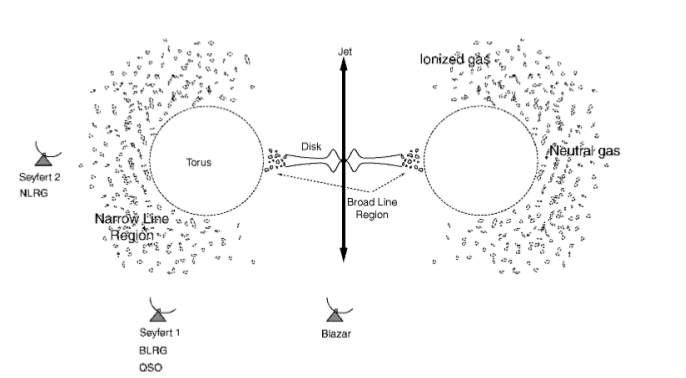
\includegraphics[scale=.5]{./figures/3_AGNs/Clasificacion_AGN}
\figcaption{\emph{Los diferentes tipos de AGNs solo dan información de que lugar del AGN se está observando \cite{schneider2006}.}}\label{fig:Tipos_AGNs_por_observador}
\end{center}


%*************************************************************************
%AGN Zoo
\section{El Enigma Central: La existencia de un Agujero Negro}
\label{sec: Enigma_centarl}
%***********************************************************************

En la teoría de los AGNs, ha existido una duda sobre el proceder de la energía que estos emanan, en especial ?`Cómo es producida? Entonces debido a esto, se plantea que dicha energía es originada por un objeto muy masivo en su interior, muy cercano al centro. El objetos propuesto lleva por nombre  Agujero Negro (BH, Black Hole), presentado como un objeto altamente compacto, que acreta materia de su alrededor. A continuación se presentan una serie de propiedades observacionales en los AGNs que dan pie a la existencia de un BH: \\

- Se encuentran fuentes de radio en AGNs que alcanzan un tamaño aproximadamente mayor a 1 Mpc. Usando esta escala de longitud es posible medir el tiempo en que ha estado activa la fuente. Para esta escala de longitud se tiene que el tiempo de vida es mayor a $10^{7}$años.

-La luminosidad de los QSOs es aproximadamente $L_{bol}\sim 10^{47}ergs$. Asumiendo que la luminosidad no cambia sustancialmente durante el tiempo de vida de la fuente, es posible medir la energía total
\begin{align}
E \gtrsim 10^{47} erg/s \times 10^{7}yr \sim 3\times 10^{61}erg\,.
\end{align}

-Para escalas de tiempo de días, se tiene que la luminosidad de los AGNs varia en un $\% 50$. Estas variabilidades permiten encontrar un límite superior para la extensión espacial de la fuente. Para una fuente puntual se tiene que la extensión es $R \lesssim 1$ día luz $\sim3\times10^{15}$cm.\\

La solución exacta de las ecuaciones de Einsten, predicen la existencia de objetos altamente compacto en cierta región del espacio-tiempo: usando la métrica de {\it{Schwarzschild}} (), se predice la existencia de un Agujero Negro (BH) estático; al usar la métrica de {\it{Kerr}} () se predice la existencia de un BH rotante. 

%---------------------------------------------------------------------
	%M
	\subsection{La Existencia de los Agujeros Negros}
	\label{subsec:Why_a_BH}
%---------------------------------------------------------------------

Usando la información observacional expuesta anteriormente y suponiendo que la producción de energía es de naturaleza gravitacional, es posible derivar la energía básica en el AGN. Suponiendo lo anterior, la forma clásica más eficiente de transformación de energía es por medio de la fusión nuclear. 

La fusión del hidrógeno, produce 8Mev/nucleon. La máxima eficiencia de fusión nuclear es $\epsilon \lesssim 0.81 \%$, donde $\epsilon$ es la fracción de masa del combustible que es convertido en energía. De acuerdo con 
\begin{align}
E=\epsilon mc^{2}\,,
\end{align}
%
la energía por fusión es $E=3\times10^{61}$. Entonces la masa que produce el combustible necesitaría ser 
\begin{align}
m=\frac{E}{\epsilon c^{2}} \sim 4\times10^{42}g\sim 2\times10^{9}M_{\odot}\,.
\end{align}

Al suponer que la naturaleza de la energía es meramente gravitacional, se tiene entonces que a medida que la materia cae dentro del BH pierde energía potencial, pero adquiere energía cinética . Al convertir la energía cinética en energía interna(calor) que será emitida en forma de radiación.

Sin embargo, los BH no son la única solución simple para las ecuaciones de Einstein. La existencia de un SMBH (Supermassive Black Hole) es posible al conocer la naturaleza de la distribución de masa compacta. También se ha encontrado evidencia observacional que ratifica la existencia de estos objetos super masivos. 

%---------------------------------------------------------------------
	%M
	\subsection{Proceso de Acreción.}
	\label{subsec:Acretion}
%---------------------------------------------------------------------

A medida que el gas cae hacia un objeto compacto, las partículas de gas pierden energía potencial que a su vez se convierte en cinética. Al conocer que el momentum angular del gas es finito, se tiene certeza que el gas no puede caer directamente hacia el objeto. A medida que este cae, siente una fricción por la interacción con las otras partículas circundantes, lo que se traduce en una transferencia de momentum, que dará como resultado la formación de un disco de acreción perpendicular al momentum angular. La fricción en el disco será la responsable de desacelerar la velocidad de rotación de las partículas, haciendo que estas caigan hacia el centro y sean acretadas por el BH.  

De acuerdo con el teorema del virial, la mitad de la energía potencial se ha cambiado en energía cinética. Por tanto, la mitad de la energía se ha convertido en energía de rotación. Así, la mitad de la energía potencial se convirtió en energía interna. 

La energía generada por la fricción dinámica en el disco, no cuenta con la suficiente energía para poder escapar de allí, pero aun así es capaz de calentar el gas y producir un engrosamiento en el disco, como en la figura (\ref{fig:Tipos_AGNs_por_observador}).


%---------------------------------------------------------------------
	%M
	\subsection{Generación de Jets.}
	\label{subsec:Generation_Jets}
%---------------------------------------------------------------------

Los lóbulos radiales son producidos por partículas cargadas eyectadas desde el centro del AGN, a velocidades relativistas. Estas partículas son aceleradas desde el núcleo en dos direcciones opuestas. El impulso es producido por la extracción de energía cinética de rotación del BH a través del mecanismo de Blandford- Znajek \cite{blandford1977}. Ver figura (\ref{fig:Modelo_interior_AGN}).% En el disco se encuentra el campo magnético  que está acoplado a este flujo de partículas. 

Al observar un AGN es inevitable ver que los jets producidos son extremadamente delgados y muy rectos. Lo cual implica  que los procesos que lo generaron ocurrieron muy al interior del disco, donde el núcleo es el responsable de colimar estos rayos de alta energía. %Es importante aclarar que este mecanismo no reproduce los flujos de materia relativista; sin embargo hay una nueva rama que pretende dar solución a este problema. La hidrodinámica es la responsable de reproducir los fenómenos con una mayor precisión, pero con el costo de poder computacional.
%
\begin{center}
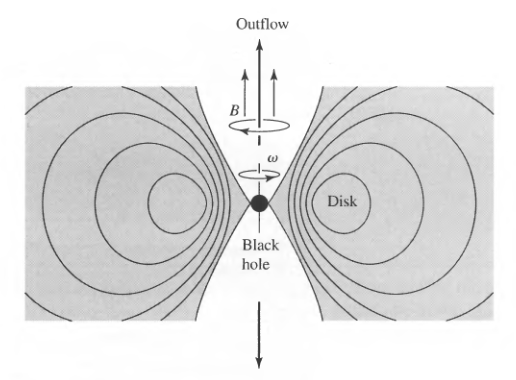
\includegraphics[scale=.5]{./figures/3_AGNs/Jets.png}
\figcaption{\emph{Bosquejo del modelo de la estructura del núcleo del AGN \cite{carroll2007}, donde se puede ver el mecanismo de Blandfort- Znajek}}\label{fig:Modelo_interior_AGN}
\end{center}

%---------------------------------------------------------------------
	%M
	\subsection{Formación de Lóbulos.}
	\label{subsec:Formation_lobules}
%---------------------------------------------------------------------

Cuando los jets expulsan las partículas altamente cargadas del núcleo, estas llevan consigo una energía cinética. A medida que se desplazan por el medio interestelar van perdiendo energía y se van desacelerando. Las partículas que van adelante del flujo de materia, son las que más siente la interacción con otras partículas y se van ralentizando, de una forma más brusca, formando un frente de choque. Este frente de choque provoca que las partículas se vaya esparciendo  de forma desordenada generando los lóbulos, como se observa en la figura (\ref{fig:Lobulos}).

\begin{center}
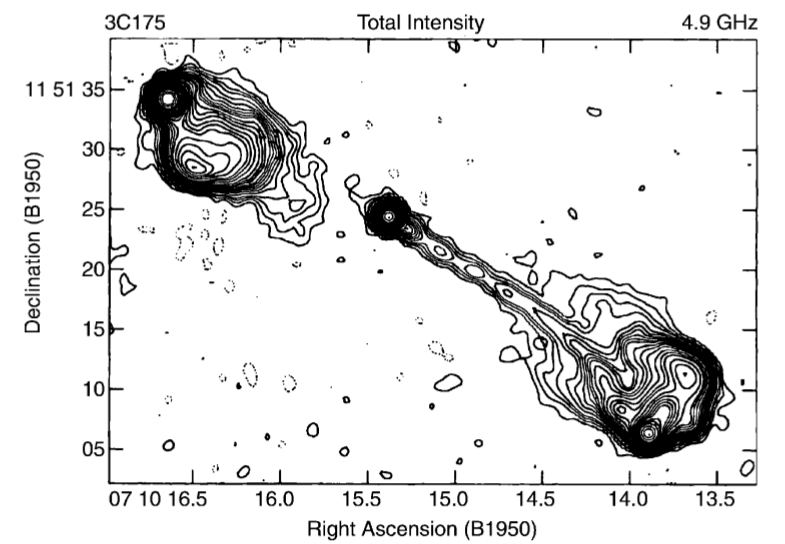
\includegraphics[scale=.3]{./figures/3_AGNs/Lobulos_y_Jets.png}
\figcaption{\emph{Simulación de un AGN\cite{schneider2006}. En la parte central se encuentra el BH, los jets son por donde se desplaza la materia y los lóbulos son los grumos donde se aglomera la materia que viene del núcleo.}}\label{fig:Lobulos}
\end{center}

%*********************************************************************
	%M
\section{Modelo Unificado}
\label{sec:Unified_models}
%*********************************************************************

Conforme a todo lo presentado, se puede identificar que los AGNs presentan cierta similitud, pero de igual manera diferencias considerables. Al conocer su naturaleza, se pretende mostrar a los AGNs como objetos con morfología equivalente, cuya diferencia radica en que son observados en lugares distintos, en los cuales se evidencian fenómenos físicos específicos del AGNs. Mirar figura (\ref{fig:Tipos_AGNs_por_observador}).

Como ya se ha dicho y mostrado los AGNs presentan propiedades en común: \\

- Todas los AGNs hospedan un SMBH en su interior. 

- Todos los AGNs tiene un disco de acreción que alimenta el BH.

- Todos los AGNs van a estar caracterizados por la masa del BH $M_{BH}$ y de la rata de acreción $\dot{m}$. $M_{BH}$ permite relacionar la luminosidad máxima del SMBH. 

- La morfología de la galaxia anfitriona también permite clasificar, como por ejemplo: Las radio galaxias están en galaxias espirales, mientras que las Seyferts en galaxias espirales.\\

Con estos criterios se pretende construir un criterio de clasificación más amplio, que permita albergar todos los tipos de AGNs.





%*************************************************************************